\chapter{Einleitung}
%Ziel des Versuchs.
\section{Kapazität des variablen Kondensators}
Allgemein ist die Kapazität eines Kondensators durch \gl{eq:cap} definiert. Für den Fall eines Plattenkondensators dessen
Platten einen runden Querschnitt besitzen und parallel zueinander stehen lässt sich seine Kapazität vereinfacht durch
\gl{eq:plattencap} ausdrücken.
\begin{equation}
    C = \frac{Q}{U}
    \label{eq:cap}
\end{equation}
%
\begin{figure}[h]
    \centering
    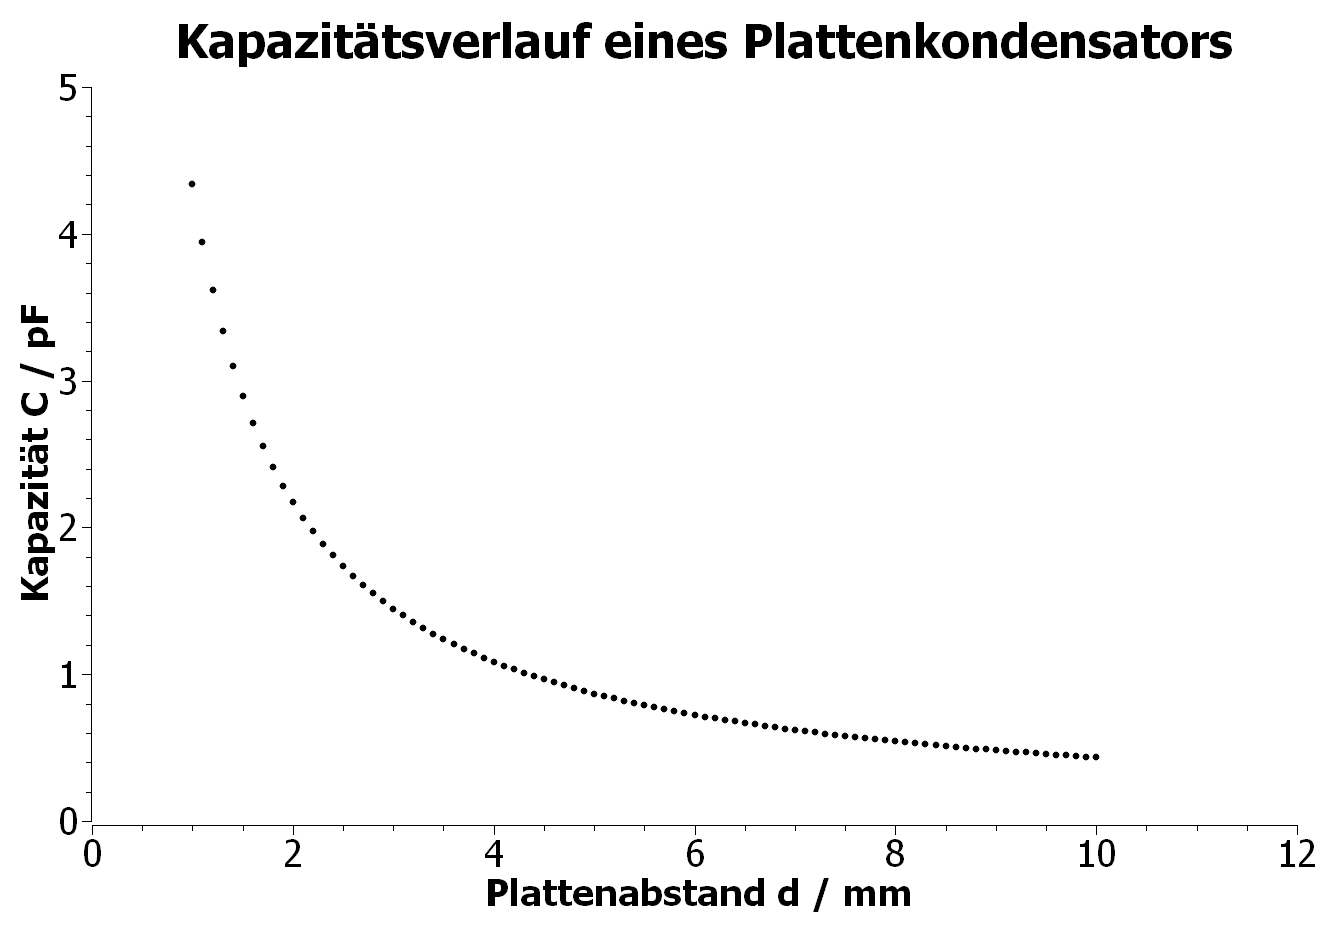
\includegraphics[width=.8\textwidth]{scidavis/kapazitaetsverlauf.jpeg}
    \caption[Kapazitätsverlauf eines Plattenkondensators]{Kapazitätsverlauf eines Plattenkondensators bei variablem Plattenabstand im Intervall \(\SI{1}{mm} \leq d \leq \SI{10}{mm}\)}
    \label{fig:kapVerlauf}
\end{figure}
%
\begin{equation}
    C = \varepsilon_0\varepsilon_r \cdot \frac{A}{d} \quad \text{und} \quad A = \frac{D^2 \pi}{4}
    \label{eq:plattencap}
\end{equation}
Hierbei ist \(\varepsilon_0\) die \textit{elektrische Feldkonstante} mit \(8,85 \cdot 10^{-12}\SI{}{\tfrac{As}{Vm}}\) \cite{Haberle.2007}
und \(\varepsilon_r\) die materialabhängige relative Permittivitätszahl. \bild{fig:kapVerlauf} zeigt den Kapazitätsverlauf
eines runden Plattenkondensators mit konstantem Durchmesser \(D = \SI{255}{mm}\), Luft als Dielektrikum (\(\varepsilon_r = 1\))
und einem Plattenabstand im Intervall \(\SI{1}{mm} \leq d \leq \SI{10}{mm}\). Es ist erkennbar, dass sich die Kapazität des Kondensators
bei größerem Plattenabstand rasch verringert und im weiteren Verlauf asymptotisch gegen \(0\) läuft.
%
%======================================================================================
%
\section{Bestimmung der Feldkonstante}
In die Form \(C_1(d^{-1}) = \varepsilon_0\varepsilon_r A \cdot d^{-1}\) gebracht lässt sich aus der Steigung des
linearisierten Kapazitätsverlaufs die Feldkonstante \(\varepsilon_0\) bestimmen.
\begin{figure}[h]
    \centering
    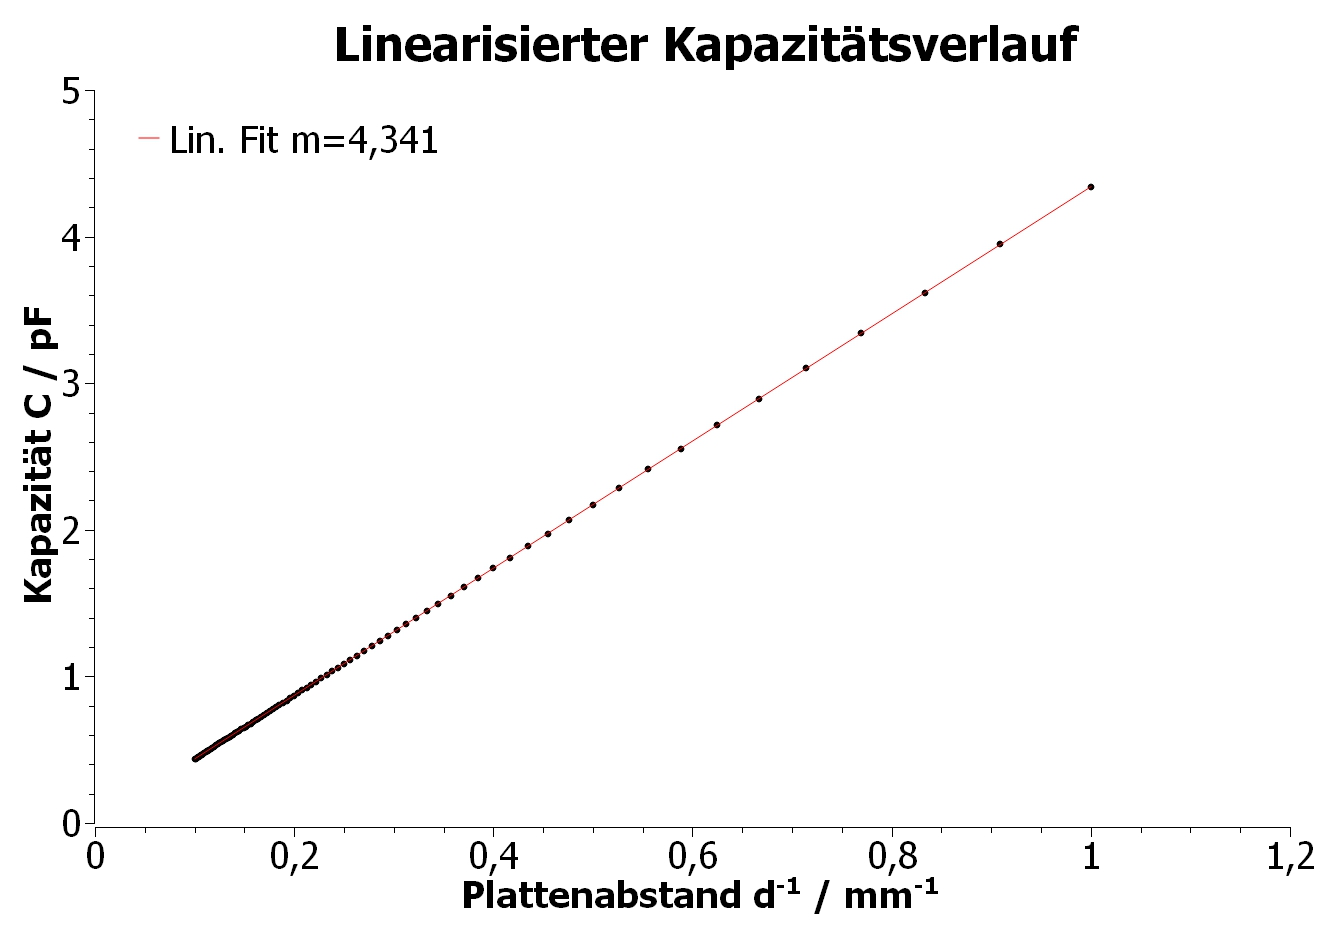
\includegraphics[width=.8\textwidth]{scidavis/linearisierter_kapazitaetsverlauf.jpeg}
    \caption[Linearisierter Kapazitätsverlauf]{Linearisierter Kapazitätsverlauf aus \bild{fig:kapVerlauf}. Mit bekannter Steigung der Ausgleichgeraden lässt sich die Feldkonstante \(\varepsilon_0\) bestimmen.}
    \label{fig:lin_kapVerlauf}
\end{figure}
\begin{align}
    m &= \varepsilon_0\varepsilon_r A \nonumber \\
    &\Leftrightarrow \nonumber \\
    \varepsilon_0 &= \frac{m}{\varepsilon_r A}
    \label{eq:e0}
\end{align}
%
%======================================================================================
%
\section{Bestimmung der Kapazität}
%
Die unbekannte Kapazität eines Kondensators \(C_1\) lässt sich mit einem einfachen Aufbau bestimmen. Der Kondensator
\(C_1\) wird an einer Konstantspannungsquelle zunächst auf eine definierte Spannung \(U_1\) geladen (siehe \bild{fig:c1laden}).
Im Gleichgewichtszustand beträgt die in \(C_1\) gespeicherte Ladung nach \gl{eq:cap}
\begin{equation}
    Q = C_1 \cdot U_1
    \label{eq:ladungc1}
\end{equation}
\begin{figure}[h]
    \centering
    \begin{minipage}[b]{.45\linewidth}
        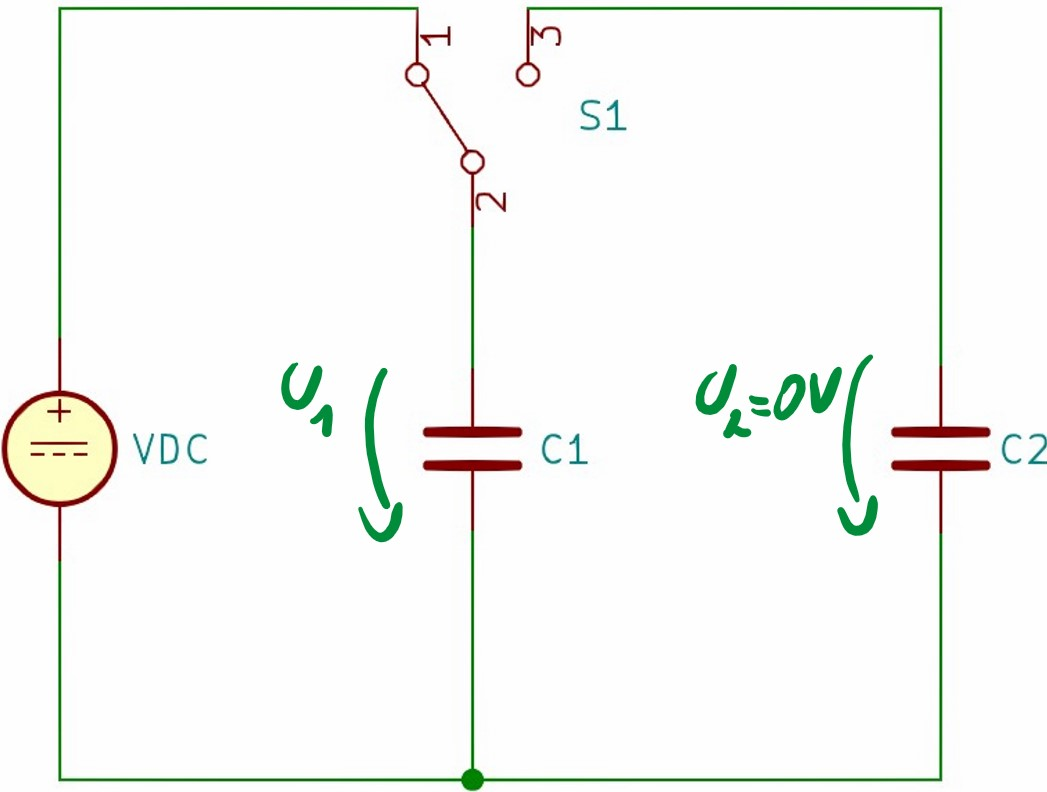
\includegraphics[width=.95\linewidth]{kicad/abbildungen/c1laden_annot.jpg}
        \caption[]{Initiales Laden des Kondensators \(C_1\).}
        \label{fig:c1laden}
    \end{minipage}
    \begin{minipage}[b]{.45\linewidth}
        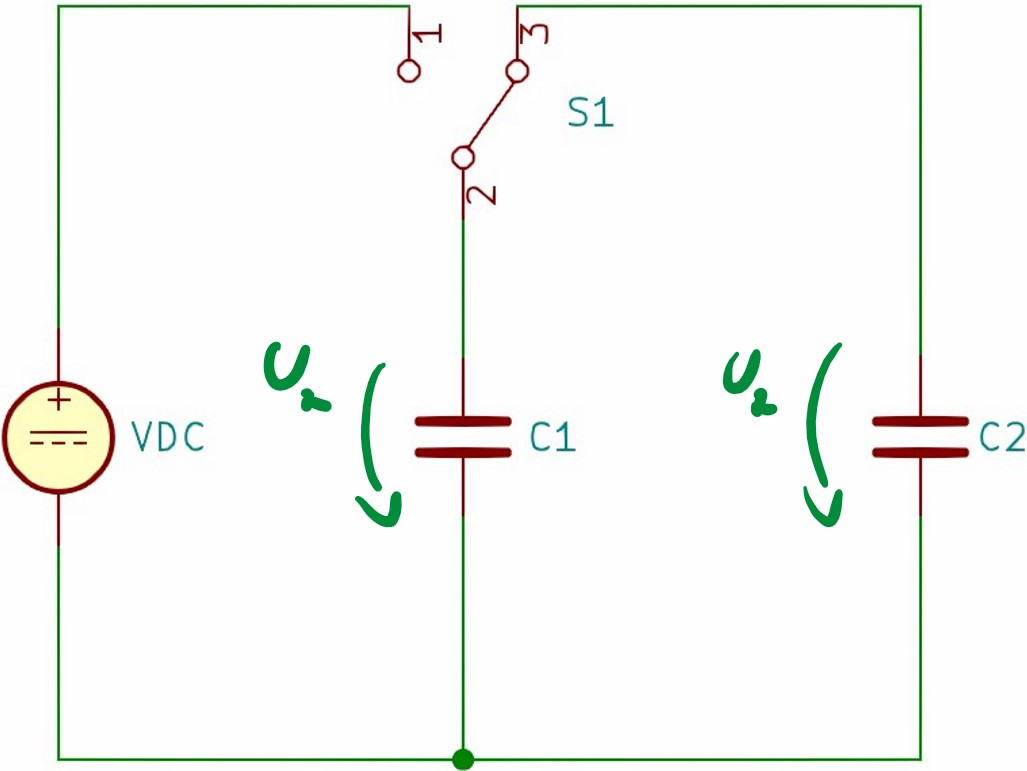
\includegraphics[width=.95\linewidth]{kicad/abbildungen/c1entladen_annot.jpg}
        \caption[]{Ladungsumverteilung von \(C_1\) hin zu \(C_2\).}
        \label{fig:c1entladen}
    \end{minipage}
\end{figure}
Wird nun \(S1\) umgeschaltet verteilt sich die in ihm gespeicherte Ladung \(Q\) um auf den nun parallel geschalteten,
anfangs vollständig entladenen Kondensator bekannter Kapazität \(C_2\). Die im System gespeicherte Gesamtladung \(Q\) bleibt
bei diesem Prozess erhalten. Für die Teilladungen gilt also
\begin{equation}
    Q = Q_1 + Q_2
    \label{eq:gesamtladung}
\end{equation}
Nachdem sich erneut ein Gleichgewicht eingestellt hat kann die nun an \(C_1\) wie \(C_2\) anliegende Spannung \(U_2 = \frac{Q_2}{C_2}\) gemessen
werden (vgl. \bild{fig:c1entladen}). Mit diesem Wissen und einsetzen von \gl{eq:ladungc1} in \gl{eq:gesamtladung} kann die Kapazität von \(C_1\) berechnet werden.
\begin{align}
    Q               &= Q_1 + Q_2 \nonumber \\
    C_1 \cdot U_1   &= C_1 \cdot U_2 + C_2 \cdot U_2 \nonumber \\
    \Leftrightarrow \quad C_1 (U_1 - U_2)                               &= C_2 \cdot U_2 \nonumber \\
    \Leftrightarrow \quad C_1                                           &= C_2 \cdot \frac{U_2}{U_1 - U_2}
    \label{eq:c1}
\end{align}
%
%==========================================================================
%
\section{Bestimmung der Dielektrizitätszahl}
Im Fall des Plattenkondensators unter Vernachlässigung von Effekten nahe der Plattenränder kann die elektrische Feldstärke
vereinfacht durch \gl{eq:feldPlatte} \cite{Halliday.2005} dargestellt werden.
\begin{equation}
    E = \frac{Q}{\varepsilon_0\varepsilon_r A}
    \label{eq:feldPlatte}
\end{equation}
Das Integral entlang der Feldlinien gibt die Potentialdifferenz oder die Spannung \(U\). Es folgt mit \gl{eq:feldPlatte}:
\begin{align}
    \int_{0}^{d} E \,\mathrm{d}s &= U = \frac{Q d}{\varepsilon_0\varepsilon_r A} \\
    &\Leftrightarrow \nonumber \\
    \frac{Q}{U} &= C = \varepsilon_0 \varepsilon_r \frac{A}{d}
    \label{eq:feldPlatte2}
\end{align}
Wird die Dielektrizitätszahl \(\varepsilon_r\) eines unbekannten Materials gesucht, kann jemand sich die Zusammenhänge
aus \gl{eq:feldPlatte2} zu Nutze machen.\par
Es sei der Raum zwischen den Platten eines Kondensators bekannter Plattenfläche \(A\), Kapazität \(C_0\) und Plattenabstand \(d\)
anfangs vollständig mit Luft gefüllt - für Luft kann \(\varepsilon_r = 1\) angenommen werden. Der Kondensator wird auf
eine Spannung geladen und im geladenen Zustand elektrisch isoliert.\par
Wird nun ein Dielektrikum zwischen die Platten des Kondensators Flächendeckend platziert, kann ein absinken der
Kondensatorspannung um den Faktor \(\varepsilon_r^{-1}\) fest gestellt werden. Da auch hier die im System gespeicherte Ladung
konstant bleibt geht damit nach \gl{eq:cap} eine Erhöhung der Kapazität einher. Die Dielektrizitätszahl des Materials
kann nun durch Vergleich der beiden Kapazitäten berechnet werden:
\begin{align}
    \frac{C_D}{C_0} &= \frac{\varepsilon_0\varepsilon_r \frac{A}{d}}{\varepsilon_0\varepsilon_{r,Luft} \frac{A}{d}} \nonumber \\
    \varepsilon_r &= \frac{C_D}{C_0} \cdot \varepsilon_{r,Luft} \nonumber \\
    &\Leftrightarrow \nonumber \\
    \varepsilon_r = \frac{C_D}{C_0} \quad &\text{für} \quad \varepsilon_{r,Luft} = 1
    \label{eq:rel_feld}
\end{align}

%\section{Gleichungen und Herleitungen}
%Herleitung der gegebenen Gl. aus den Grundgleichungen.
